\section{根付き全域森問題}\label{chap:problem}

配電網(図\ref{fig:dnet})を表すグラフを図\ref{fig:dnetgraph}に示す.
なお,スイッチの開閉状態はここでは考慮しないものとする.

%%%%%%%%%%%%%%%%%%%%%%%%%
\begin{figure}[htbp]
 \centering
 \scalebox{0.8}{%%%%%%%%%%%%%%%%%%%%%%%%%%%%%%%%%%%%%%%%%%%%%%%%%%
% 配電網 -> グラフ (第2章で使う)
%%%%%%%%%%%%%%%%%%%%%%%%%%%%%%%%%%%%%%%%%%%%%%%%%%

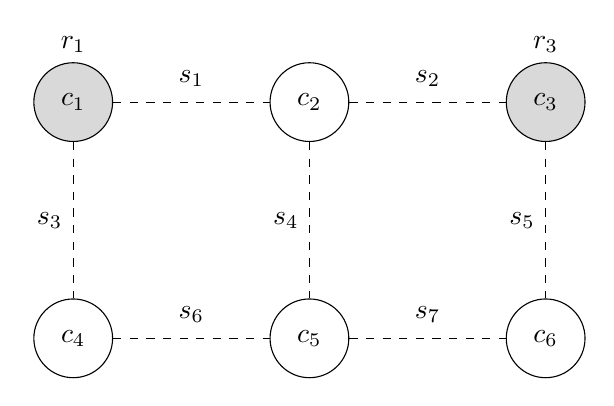
\begin{tikzpicture}[x=1.5cm,y=1.5cm]

 % 設定
 \tikzset{root/.style={circle,draw=black,fill=gray!30,minimum size=1cm}}
 \tikzset{node/.style={circle,draw=black,minimum size=1cm}}
 
 % 補助線
 % \draw [help lines,blue,step=2cm] (-3,0) grid (3,-3);

 % root %
 \node[root] at (-2,0) (1){$c_1$};
 \node[above=0.5cm] at (1) {$r_1$};
 \node[root] at (2,0) (3){$c_3$};
 \node[above=0.5cm] at (3) {$r_3$};

 % node %
 \node[node] at (0,0) (2){$c_2$};
 \node[node] at (-2,-2) (4){$c_4$};
 \node[node] at (0,-2) (5){$c_5$};
 \node[node] at (2,-2) (6){$c_6$};

 % 繋がっていない辺は破線
 \foreach \u / \v in {2/3, 2/5, 4/5}
 \draw [dashed] (\u) -- (\v);
 % 繋がってる辺は実線
 \foreach \u / \v in {1/2, 1/4, 3/6, 5/6}
 \draw [dashed] (\u) -- (\v);

 % スイッチ switch %
 \node at (-1,0.2) {$s_1$};
 \node at (1,0.2) {$s_2$};
 \node at (-2.2,-1) {$s_3$};
 \node at (-0.2,-1) {$s_4$};
 \node at (1.8,-1) {$s_5$};
 \node at (-1,-1.8) {$s_6$};
 \node at (1,-1.8) {$s_7$};
 %

\end{tikzpicture}

%%%%%%%%%%%%%%%%%%%%%%%%%%%%%%%%%%%%%%%%%%%%%%%%%%%%%%%%%%
%%% Local Variables:
%%% mode: japanese-latex
%%% TeX-master: paper.tex
%%% End:
}
 \caption{配電網(図\ref{fig:dnet})を表すグラフ}
 \label{fig:dnetgraph}
\end{figure}
%%%%%%%%%%%%%%%%%%%%%%%%%

図\ref{fig:dnet}における需要家$\{c_1,\ldots,c_6\}$は,\textbf{ノード}に対応し,
スイッチ$\{s_1,\ldots,s_7\}$は,\textbf{辺}に対応している.
図中の色付きノード$\{c_1,c_3\}$は変電所と直接繋がっている需要家を意味しており,
\textbf{根}を表している.
また,根はノードの添字を用いて$\{r_1,r_3\}$のように表す.

\comment{ここまで追加しました.}

\theoremstyle{definition}
\newtheorem*{definition*}{定義}

根付き全域森は以下のように定義される~\cite{Minato:dnet:netuki}.
\begin{definition*}
  グラフ$G=(V,E)$と,根と呼ばれる$V$上のノードの集合が与えられたとする.
  このとき,$G$上の根付き全域森とは,以下の制約を満たす$G$の部分グラフ
  $G'=(V,E'), E' \subseteq E$ である.
  \begin{enumerate}
  \item $G'$はサイクルを持たない.(非閉路制約)
  \item $G'$の各連結成分は,ちょうど1つの根を含む.(根付き連結制約)
  \end{enumerate}
本稿では,与えられたグラフ$G$から,根付き全域森
$G'$を求める部分グラフ探索問題を\textbf{根付き全域森問題}と呼ぶ.
\end{definition*}

%%%%%%%%%%%%%%%%%%%%%%%%%
\begin{figure}[htbp]
  \centering
  \scalebox{0.8}{%%%%%%%%%%%%%%%%%%%%%%%%%%%%%%%%%%%%%%%%%%%%%%%%%%
% 根付き全域森 (第2章で使う)
%%%%%%%%%%%%%%%%%%%%%%%%%%%%%%%%%%%%%%%%%%%%%%%%%%

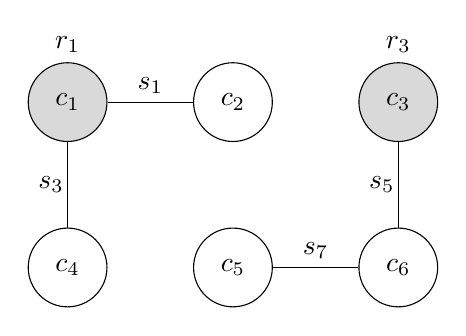
\begin{tikzpicture}[x=1.5cm,y=1.5cm,scale=0.7]

 % 設定
 \tikzset{root/.style={circle,draw=black,fill=gray!30,minimum size=1cm}}
 \tikzset{node/.style={circle,draw=black,minimum size=1cm}}
 
 % 補助線
 % \draw [help lines,blue,step=2cm] (-3,0) grid (3,-3);

 % root %
 \node[root] at (-2,0) (1){$c_1$};
 \node[above=0.5cm] at (1) {$r_1$};
 \node[root] at (2,0) (3){$c_3$};
 \node[above=0.5cm] at (3) {$r_3$};

 % node %
 \node[node] at (0,0) (2){$c_2$};
 \node[node] at (-2,-2) (4){$c_4$};
 \node[node] at (0,-2) (5){$c_5$};
 \node[node] at (2,-2) (6){$c_6$};

 % 繋がっていない辺は破線
 %\foreach \u / \v in {2/3, 2/5, 4/5}
 %\draw [dashed] (\u) -- (\v);
 % 繋がってる辺は実線
 \foreach \u / \v in {1/2, 1/4, 3/6, 5/6}
 \draw (\u) -- (\v);

 % スイッチ switch %
 \node at (-1,0.2) {$s_1$};
 %\node at (1,0.2) {$s_2$};
 \node at (-2.2,-1) {$s_3$};
 %\node at (-0.2,-1) {$s_4$};
 \node at (1.8,-1) {$s_5$};
 %\node at (-1,-1.8) {$s_6$};
 \node at (1,-1.8) {$s_7$};
 %

\end{tikzpicture}

%%%%%%%%%%%%%%%%%%%%%%%%%%%%%%%%%%%%%%%%%%%%%%%%%%%%%%%%%%
%%% Local Variables:
%%% mode: japanese-latex
%%% TeX-master: paper.tex
%%% End:
}\\[1em]
  \scalebox{0.8}{%%%%%%%%%%%%%%%%%%%%%%%%%%%%%%%%%%%%%%%%%%%%%%%%%%
% 根付き全域森 (第2章で使う)
%%%%%%%%%%%%%%%%%%%%%%%%%%%%%%%%%%%%%%%%%%%%%%%%%%

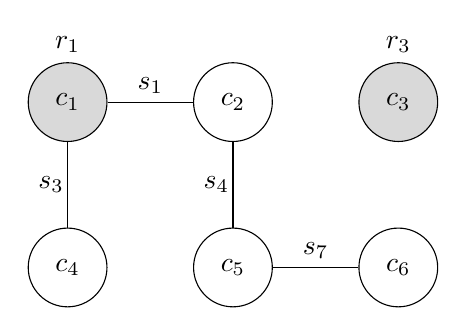
\begin{tikzpicture}[x=1.5cm,y=1.5cm,scale=0.7]

 % 設定
 \tikzset{root/.style={circle,draw=black,fill=gray!30,minimum size=1cm}}
 \tikzset{node/.style={circle,draw=black,minimum size=1cm}}
 
 % 補助線
 % \draw [help lines,blue,step=2cm] (-3,0) grid (3,-3);

 % root %
 \node[root] at (-2,0) (1){$c_1$};
 \node[above=0.5cm] at (1) {$r_1$};
 \node[root] at (2,0) (3){$c_3$};
 \node[above=0.5cm] at (3) {$r_3$};

 % node %
 \node[node] at (0,0) (2){$c_2$};
 \node[node] at (-2,-2) (4){$c_4$};
 \node[node] at (0,-2) (5){$c_5$};
 \node[node] at (2,-2) (6){$c_6$};

 % 繋がっていない辺は破線
 %\foreach \u / \v in {2/3, 2/5, 4/5}
 %\draw [dashed] (\u) -- (\v);
 % 繋がってる辺は実線
 \foreach \u / \v in {1/2, 1/4, 2/5, 5/6}
 \draw (\u) -- (\v);

 % スイッチ switch %
 \node at (-1,0.2) {$s_1$};
 %\node at (1,0.2) {$s_2$};
 \node at (-2.2,-1) {$s_3$};
 \node at (-0.2,-1) {$s_4$};
 %\node at (1.8,-1) {$s_5$};
 %\node at (-1,-1.8) {$s_6$};
 \node at (1,-1.8) {$s_7$};
 %

\end{tikzpicture}

%%%%%%%%%%%%%%%%%%%%%%%%%%%%%%%%%%%%%%%%%%%%%%%%%%%%%%%%%%
%%% Local Variables:
%%% mode: japanese-latex
%%% TeX-master: paper.tex
%%% End:
}
  \caption{根付き全域森の出力例 (2つ)}
  \label{fig:netuki}
\end{figure}
%%%%%%%%%%%%%%%%%%%%%%%%%

根付き全域森の例を図\ref{fig:netuki}に示す.
根付き全域森は,各連結成分が必ずちょうど1つの根をもつ木構造を
形成することで,非閉路制約と根付き連結制約を満たす.
図~\ref{fig:netuki}の上側は,図~\ref{fig:dnet}の配電網問題の解に
対応している.
根付き全域森問題には解が複数存在し得る.
例えば,図~\ref{fig:netuki}の下側は,
ある連結成分が根のみとなる場合を表している.

%%% Local Variables:
%%% mode: japanese-latex
%%% TeX-master: "paper"
%%% End:
